\documentclass[12pt,a4paper,oneside]{article}

% This first part of the file is called the PREAMBLE. It includes
% customizations and command definitions. The preamble is everything
% between \documentclass and \begin{document}.

\usepackage[margin=1in]{geometry}  % set the margins to 1in on all sides
\usepackage{graphicx}              % to include figures
\usepackage{amsmath}               % great math stuff
\usepackage{amsfonts}              % for blackboard bold, etc
\usepackage{amsthm}                % better theorem environments
\usepackage[english]{babel}
\usepackage[square, numbers]{natbib}
\usepackage[T1]{fontenc}
\usepackage[utf8]{inputenc}
\usepackage{lmodern}
\usepackage{amssymb}
\usepackage{authoraftertitle}
\usepackage{hyperref}
\usepackage{multicol}
\usepackage{caption}
\usepackage{subcaption}
\usepackage{placeins}
\usepackage{setspace}
%\usepackage{indentfirst}

\onehalfspace
%\singlespace

% Author
\author{Ondrej Škopek\\
Faculty of Mathematics and Physics\\
Charles University in Prague\\
\texttt{\href{mailto:oskopek@matfyz.cz}{oskopek@matfyz.cz}}}

\title{Individual software project -- specification}

%\date{3. mája 2015}
\date{\today}

% hyperref

\hypersetup{
    bookmarks=true,         % show bookmarks bar?
    unicode=true,          % non-Latin characters in Acrobat’s bookmarks
    pdftoolbar=true,        % show Acrobat’s toolbar?
    pdfmenubar=true,        % show Acrobat’s menu?
    pdffitwindow=true,     % window fit to page when opened
    pdfstartview={FitV},    % fits the width of the page to the window
    pdftitle={\MyTitle},    % title
    pdfauthor={\MyAuthor},     % author
    pdfsubject={\MyTitle},   % subject of the document
    pdfcreator={\MyAuthor},   % creator of the document
    pdfproducer={\MyAuthor}, % producer of the document
    pdfkeywords={software} {project} {planning} {automated planning} {java} {javafx} {ipc} {transport domain}, % list of keywords
    pdfnewwindow=true,      % links in new PDF window
    colorlinks=false,       % false: boxed links; true: colored links
    linkcolor=red,          % color of internal links (change box color with linkbordercolor)
    citecolor=green,        % color of links to bibliography
    filecolor=magenta,      % color of file links
    urlcolor=cyan,           % color of external links
}


% various theorems, numbered by section

\newtheorem{thm}{Theorem}[section]
\newtheorem{lem}[thm]{Lemma}
\newtheorem{obsv}[thm]{Observation}
\newtheorem{cor}[thm]{Corollary}
\newtheorem{conj}[thm]{Conjecture}

\DeclareMathOperator{\id}{id}

\newcommand{\TODO}[1]{{\textbf{TODO:} #1}} % for TODOs
\newcommand{\comment}[1]{} % for comments

\newcommand{\dist}{\text{dist}} % distance function
\newcommand{\bd}[1]{\mathbf{#1}} % for bolding symbols 
\newcommand{\RR}{\mathbb{R}}      % for Real numbers
\newcommand{\ZZ}{\mathbb{Z}}      % for Integers
\newcommand{\col}[1]{\left[\begin{matrix} #1 \end{matrix} \right]}
\newcommand{\comb}[2]{\binom{#1^2 + #2^2}{#1+#2}}

\begin{document}
\maketitle

\begin{abstract}
\end{abstract}

\section{Prehľad}
\section{}

\FloatBarrier
\begin{figure}
        \centering
        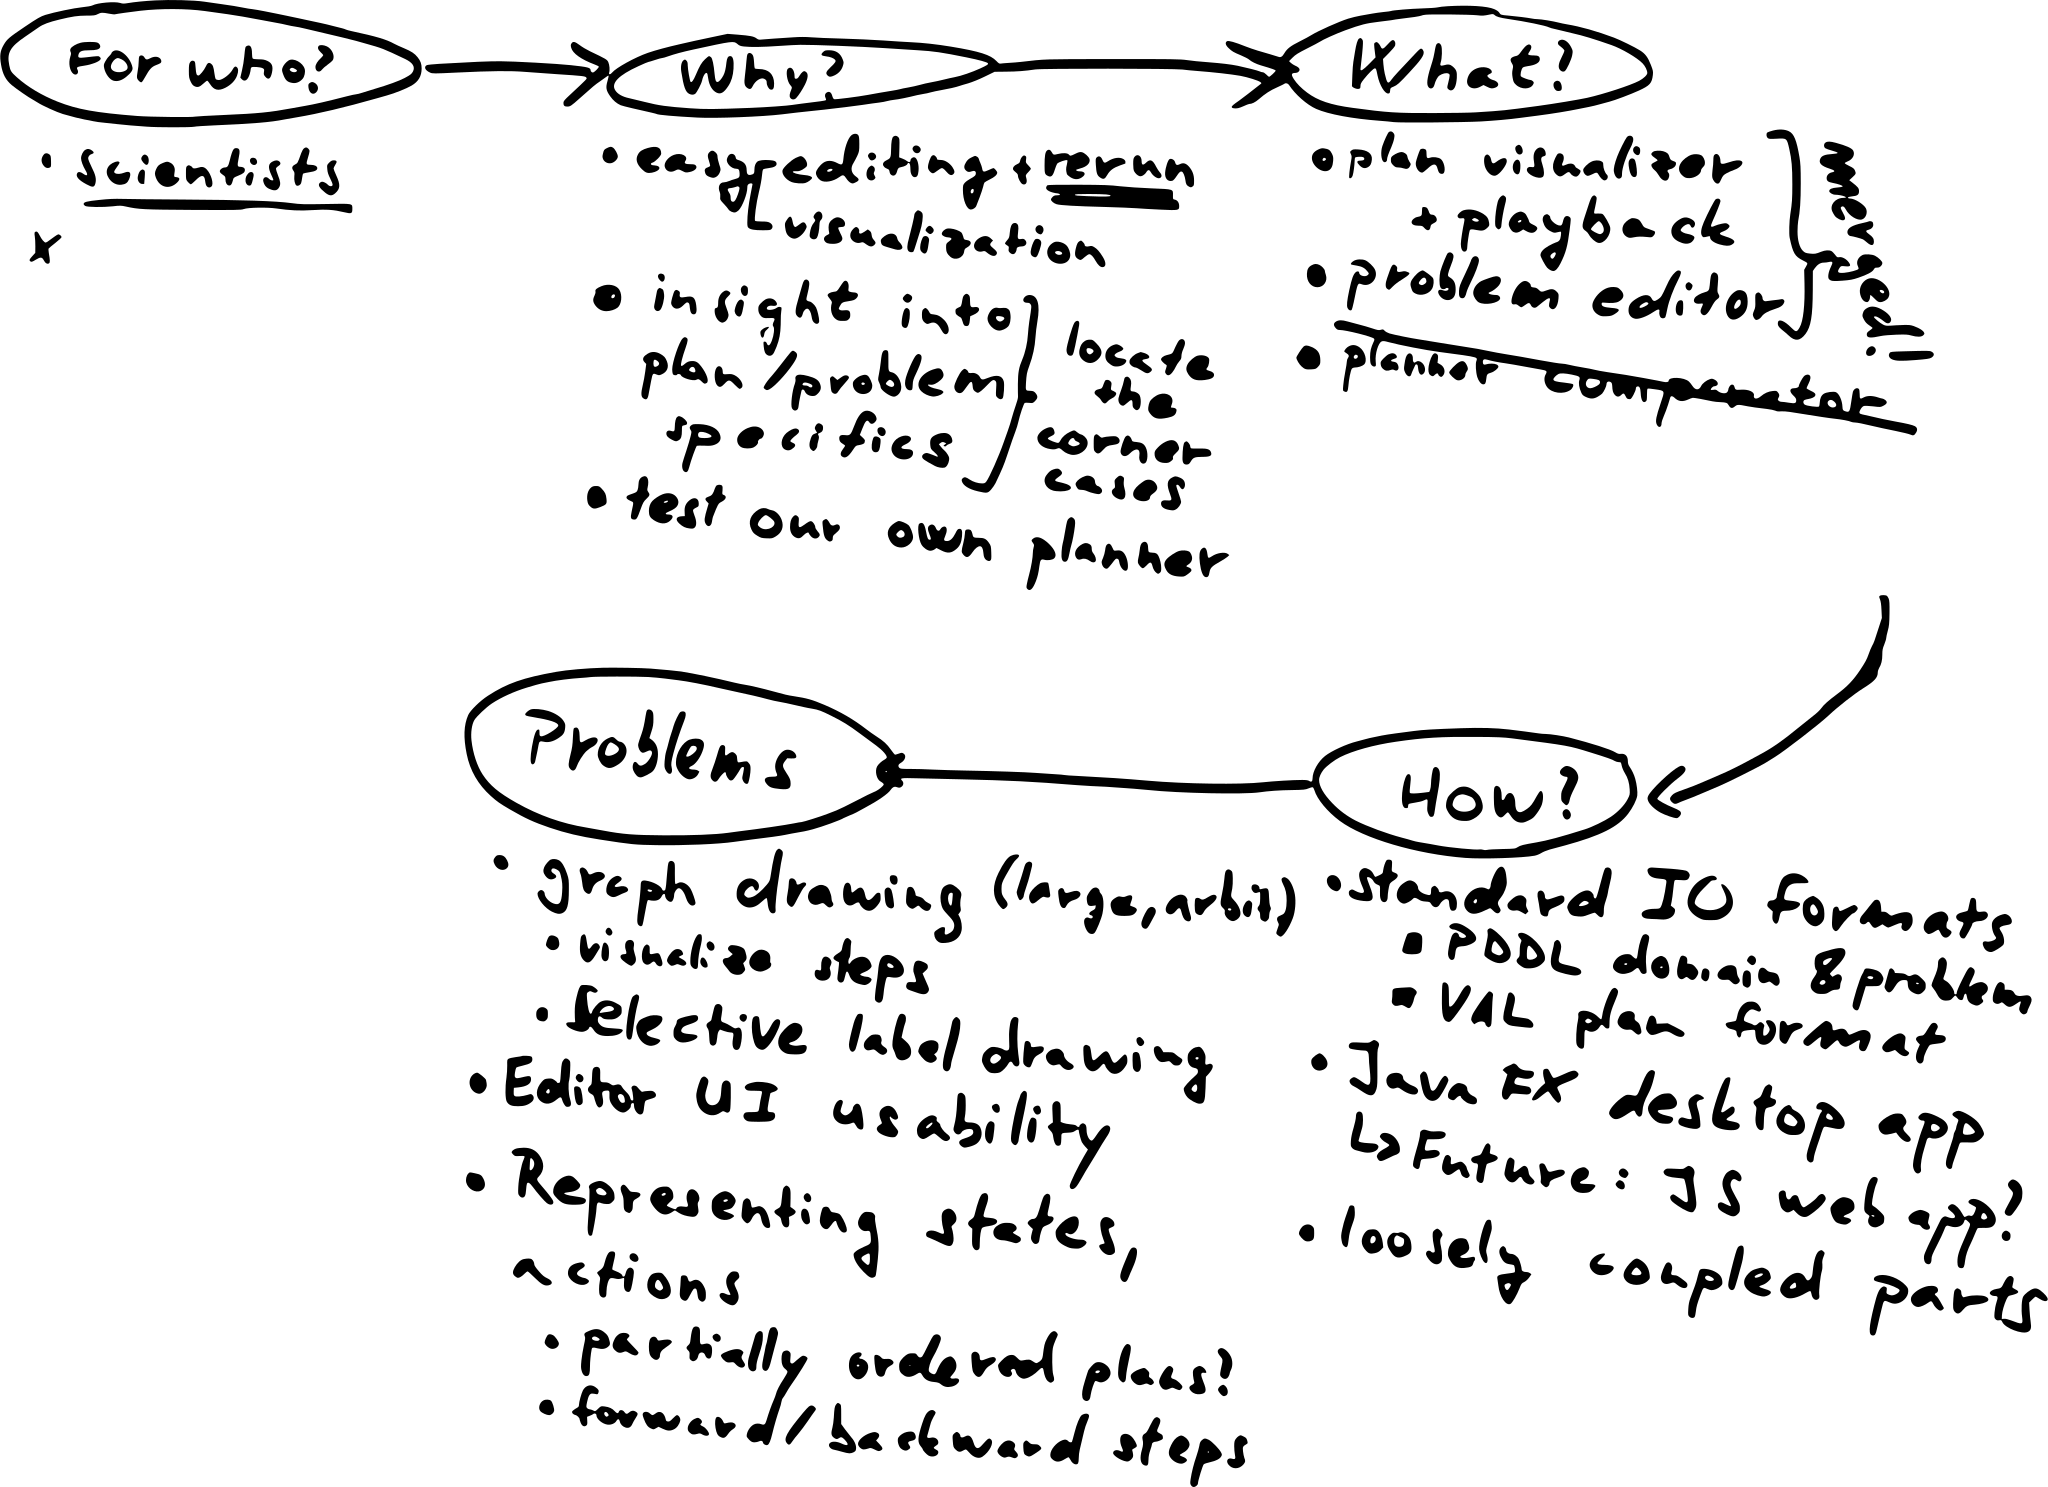
\includegraphics[width=0.8\textwidth]{../data/img/pdf/spec}
        \caption{Mindmap}
        \label{fig:mindmap}
\end{figure}
\begin{figure}
        \centering
        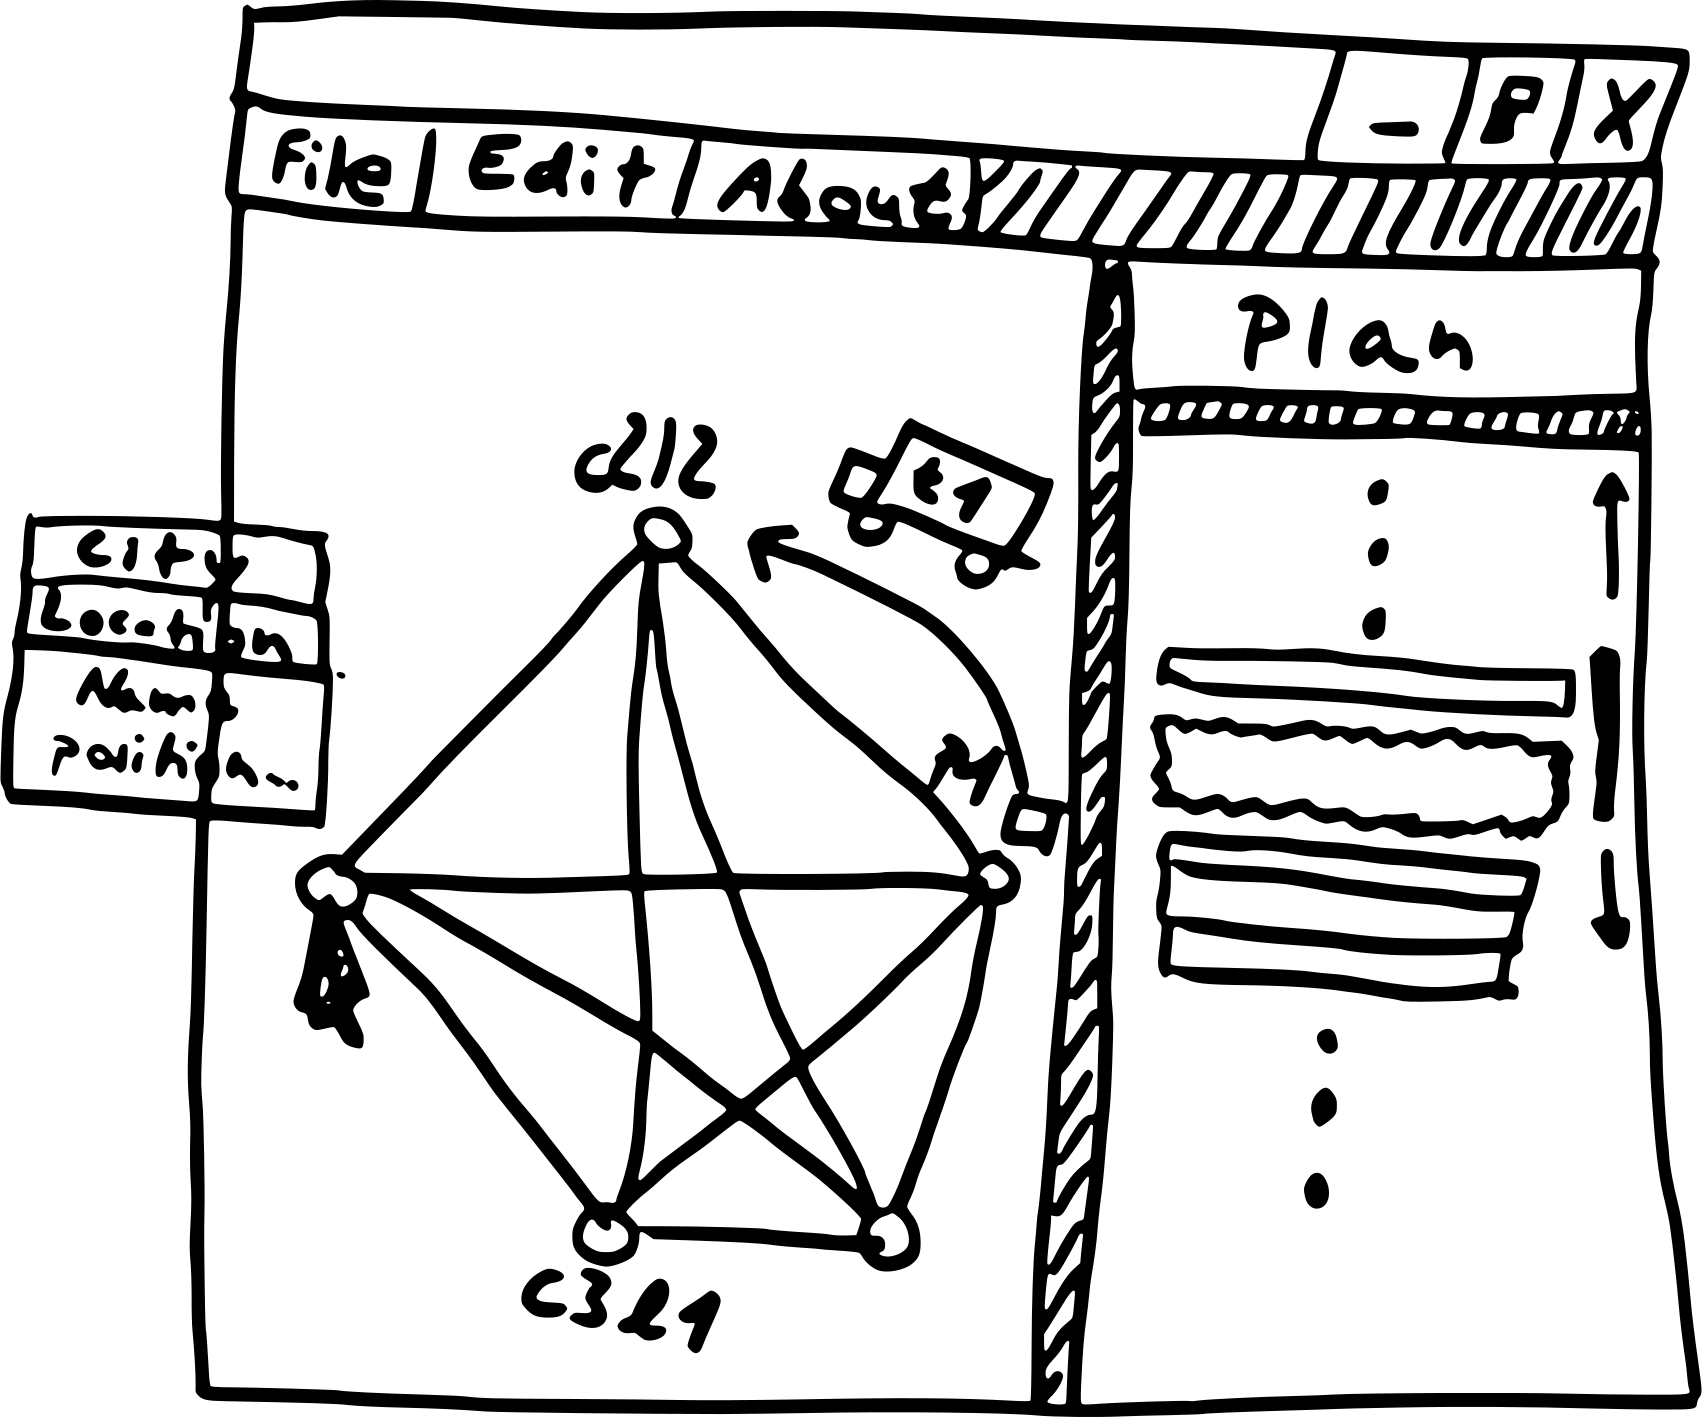
\includegraphics[width=0.8\textwidth]{../data/img/pdf/gui}
        \caption{Abstract GUI prototype}
        \label{fig:gui}
\end{figure}

\FloatBarrier


\textbf{Questions}:
\begin{itemize}
    \item Do we do temporal transport too? (petrol-stations)
    \item Is it safe to assume that symmetric edges are weight-symmetric? (all datasets have this)
\end{itemize}

Ending notes\footnote{Hand-drawn image conversion courtesy of the wonderful project cartoonist: \url{https://github.com/honzajavorek/cartoonist}}

















\comment{
\subsection{Intervalové vyhľadávanie}\label{rangesearch}

Intervalové vyhľadávanie, anglicky Range Search, je formalizácia problému vyhľadávania všetkých bodov priestoru, ktoré patria danému podpriestoru, určenom intervalovým objektom. Intervalovým objektom môže byť ľubovolný objekt vymedzujúci nejaký ,,objem`` v $k$-dimenzionálnom priestore, typicky obdĺžniky, polpriestory alebo gule.
Formálne zavedieme problém následovne \citep{agarwal97}:

\begin{quotation}
\noindent
Buď $M$ množina bodov priestoru $\mathcal{P}$ a $R$ intervalový objekt (vstup operácie \textsc{Search}).\\
Nájdi všetky body z $M$ také, ktoré patria intervalovému objektu $R$:\\ 
$X' = \{x \in M : x \in R\}$
\end{quotation}

V rámci vyhľadávania bodov z priestoru vymedzeného daným intervalovým objektom sa dajú zadefinovať rôzne iné podotázky:
\begin{itemize}
\item optimalizačné -- body so špeciálnou vlastnosťou (napr.~maximalizácia prvej súradnice)
\item počítacie -- počet takýchto bodov
\item prázdnosť -- existuje taký bod?
\end{itemize}

Vzhľadom na konkrétnu podotázku sa väčšinou dá použiť jednoduchšia/rýchlejšia datová štruktúra.

\subsection{Podobnostné vyhľadávanie}\label{simsearch}

Podobnostné vyhľadávanie, anglicky Nearest Neighbor Search (NNS), je formalizácia optimalizačného problému nájdenia najbližších (alebo najpodobnejších) bodov k zadanému bodu. Formálne sa problém zavádza následovne \citep{knuth73}: 

\begin{quotation}
\noindent
Buď $M$ množina bodov v priestore $\mathcal{P}$ a vstupný bod $x \in \mathcal{P}$.\\
Buď $\sim$ podobnostná funkcia $\sim: \mathcal{P}^2 \to \mathbb{R}$.\\
Nájdi najbližší bod $x' \in M$ ku $x$, teda: $$x' = \min_{y \in M} \{\sim(x, y)\}$$
\end{quotation}

Funkcia $\sim(x, y)$, vyjadruje teda nepriamu mieru ,,podobnosti`` (čím podobnejšie body, tým menšia funkcia). Zovšeobecnenie tohto problému je hľadanie $k$-najpodobnejších bodov ($k$-nearest neighbor search). Cieľom tohto problému je nájdenie množiny bodov veľkosti $k$, ktoré sú z danej množiny $M$ najbližšie ku $x$.

Existuje viacero algoritmov, ktoré tento problém riešia: lineárne prehľadávanie, rôzne metódy rozdeľovania na podpriestory, atď. My sa budeme zaoberať vlastnosťami datových štruktúr určených na zrýchlenie opakovaných použití takýchto algoritmov.

\section{Datové štrukúry}

V následujúcich sekciach stručne zavedieme najčastejšie používané datové štruktúry a zhrnieme ich výhody a nevýhody.

\subsection{$k$-d strom}\label{kdtree}

$k$-d strom ($k$-dimenzionálny strom) (\citet{Bentley75}) je binárny strom, v ktorom každý list je bod v priestore. 
Každý interný vrchol reprezentuje nadrovinu, ktorá rozdeľuje priestor na dve časti. Body vľavo od nadroviny sú v ľavom podstrome, body vpravo v pravom. Rovina sa volí následovne:
Zvolíme jednu z osí a hodnotu na nej. Tieto dva údaje asociujeme s daným interným vrcholom. Reprezentovaná nadrovina je kolmá na túto os, prechádzajúca danou hodnotou na osi, teda jednoznačne určená.

Z konštrukcie vyplýva, že operácie \textsc{Insert} a \textsc{Delete} majú zložitosť $O(\log n)$. Pamäťová zložitosť je triviálne $O(n)$. \citet{liberty13} rozoberá detailne zložitosť operácie \textsc{Search} s ohľadom na dimenzionalitu dát v $k$-d stromoch.

Z jeho výsledkov vyplýva, že použitie $k$-d stromov na podobnostné vyhľadávanie je vo veľkých dimenziach neoptimálne: počet bodov uložených v strome $n$ by rozhodne mal byť $n \gg 2^k$, inak je zložitosť asymptoticky rovnaká ako hľadanie hrubou silou \citep{indyk04} (lineárna), respektíve, zložitosť je exponenciálna vzhľadom na počet dimenzií.

Ďaľšia nevýhoda $k$-d stromov spočíva v tom, že na udržiavanie vlastnosti logaritmického vyhľadávania potrebujeme až $O(n\log n)$ operácií \citep{Bentley75}, teda asymptoticky rovnako ako keby sme strom vyvažovali vždy odznova.

Pre porovnanie, intervalové vyhľadávanie v $k$-d stromoch má najhoršiu zložitosť $O(kn^{1-\frac{1}{k}})$, teda polynomiálnu vzhľadom k počtu dimenzií \citep{lee77}. $k$-d stromy sú preto veľmi výhodné na použitie pri intervalovom vyhľadávaní.

\subsection{Range strom}\label{rangetree}

Range stromy zaviedol \citet{Bentley79} ako alternatívu ku $k$-d stromom určeným na intervalové vyhľadávanie s lepšou časovou zložitosťou na vyhľadávanie, ale horšou pamäťovou zložitosťou. Pre porovnanie, v Range stromoch trvá \textsc{Search} $O(\log^d n + k)$ s pamäťou $O(n \log^{d-1} n)$, kde $d$ je dimenzia daných dát.

Chazelle neskôr upravil pamäťovú zložitosť na $O\left(\left(\frac{\log n}{\log \log n}\right)^{d-1}\right)$\citep{chazelle90p1}
a časovú zložitosť vyhľadávania na $O(\log^{(d-1+\varepsilon)} n)$\citep{chazelle90p2} pre pevné $\varepsilon > 0$.

\subsection{$R$-strom}\label{rtree}

$R$-strom (rectangle tree, obdĺžnikový strom), ktorý naopak urýchľuje podobnostné vyhľadávanie zaviedol vo svojej práci \citet{Guttman84}.
Kľučovou myšlienkou je združovanie bodov do skupín a ich následná reprezentácia najmenším obdĺžnikom, ktorý ich všetky obsahuje. V listoch sa teda nachádzajú degenerované obdĺžniky obsahujúce iba jeden bod. Celkovo je strom vyvážený, teda všetky listy sa nachádzajú v rovnakej hĺbke.

Vyhľadávanie je založené na princípe pretínania vyhľadávacej otázky s obdĺžnikom v danom vrchole stromu: Ak sa nepretne vyhľadávaný obdĺžnik s obdĺžnikom vo vrchole, nemôže sa pretať ani so žiadnym z bodov, ktoré reprezentuje.

$R$-stromy nezaručujú vhodnú zložitosť v najhoršom prípade, ale na reálnych dátach fungujú preukázatelne \citep{Hwang03} dobre. Existuje varianta $R$-stromov, tzv.~prioritné $R$-stromy, ktoré majú dokazateľne optimálnu zložitosť v najhoršom prípade, ale v praxi sa nepoužívajú kvôli zložitosti implementácie.

Vzhľadom k viacdimenzionálnemu podobnostnému vyhľadávaniu, ako ukázal \citet{brinkhoff93}, 
$k$ najpodobnejších bodov sa dá nájsť v $R$-stromoch rýchlo, pomocou tzv.~spatial joins, teda ,,zjednotení v priestore`` (naprieč dimenziami), ktoré vedia $R$-stromy robiť dostatočne rýchlo. V tomto ohľade dokáže rýchlosť ešte viac vylepšiť následujúca podobná datová štruktúra, $R^*$-strom.

\subsection{$R^*$-strom}\label{rstartree}

\FloatBarrier

Ako variantu $R$-stromov s lepšou zložitosťou vyhľadávania za cenu pomalšej výstavby ho zaviedli \citet{Beckmann90}.

Skúmali vplyv rozdeľovania a pokrytia dát obdĺžnikmi v $R$-strome na rýchlosť následného vyhľadávania. Pomocou rôznych techník zmenšovania prekryvu jednotlivých obdĺžnikov vo vrcholoch zlepšili konštanty zložitosti operácie \textsc{Search} v priemernom prípade (najhorší prípad je identický s $R$-stromom) na polovičku (približne, pre detailny rozbor viď záver práce originálnych autorov \citet{Beckmann90}).

Podľa pozorovania, ktoré hovorí, že štruktúra $R$-stromu veľmi závisí od poradia vkladania bodov zmenili prístup k pretečeniu vrcholu:
opakovane vkladajú okrajové obdĺžniky z pretečeného obdĺžniku.
Tento postup vedie postupne k optimálnejšiemu stromu (body sú viac združené do skupín, teda sa dajú pokryť menším počtom obdĺžnikov) a vznikajú pravidelnejšie obdĺžniky.
Nevýhodou je, že opakovaným vkladaním sa zvyšujú časové nároky na údržbu stromu.

Rôzne rozdelenia na obdĺžniky sa dajú veľmi dobre vizualizovať v nižších dimenziach. Na obrázku \ref{fig:Splits} vidíme rôzne stratégie pre umiestnovanie bodov do obdĺžnikov vo vrcholoch $R$-stromu. Vidíme, že $R^*$-strom dokáže najlepšie zamedziť prekryvom, a preto je najvhodnejší pre praktické aplikácie, napriek vyššie spomenutým nevýhodám a implementačnej zložitosti.

\begin{figure}
        \centering
        \begin{subfigure}[b]{0.3\textwidth}
                \includegraphics[width=\textwidth]{../data/img/Zipcodes-Germany-GuttmanRTree.pdf}
                \caption{Guttmanov $R$-strom \citep{RTreeSplitImg}}
                \label{fig:RTreeSplit}
        \end{subfigure}
        ~ %add desired spacing between images, e. g. ~, \quad, \qquad, \hfill etc.
          %(or a blank line to force the subfigure onto a new line)
        \begin{subfigure}[b]{0.31\textwidth}
                \includegraphics[width=\textwidth]{../data/img/Zipcodes-Germany-AngTanSplit.pdf}
                \caption{Ang-Tan \citep{ang97} a $R$-strom \citep{AngTanSplitImg}}
                \label{fig:AngTanSplit}
        \end{subfigure}
        ~ %add desired spacing between images, e. g. ~, \quad, \qquad, \hfill etc.
          %(or a blank line to force the subfigure onto a new line)
        \begin{subfigure}[b]{0.3\textwidth}
                \includegraphics[width=\textwidth]{../data/img/Zipcodes-Germany-RStarTree.pdf}
                \caption{$R^*$-strom \citep{RStarTreeSplitImg}}
                \label{fig:RStarTreeSplit}
        \end{subfigure}%
        \caption{Rozdelenia na obdĺžniky podľa rôznych heuristík na databáze nemeckých poštových smerovacích čísel}\label{fig:Splits}
\end{figure}

\FloatBarrier

\subsection{$R^+$-strom}\label{rplustree}

Autori \citet{Sellis87} ďalšej varianty $R$-stromu, tzv.~$R^+$-stromu, úpravami znížili počet prístupov k súborovému systému pri vyhľadávaní súborov o 50\%. Hlavný rozdiel oproti Guttmanovmu $R$-stromu je zníženie počtu prekryvov v interných vrcholoch stromu, čo má za následok o málo rýchlejšie vyhľadávanie pri veľkom objeme dát. Hlavná aplikácia tohoto prístupu je v databázach.

\subsection{Pokrývací strom}\label{covertree}

Pokrývací strom (Cover tree) bol zavedený autorom \citet{Clarkson06} špeciálne na zrýchlenie podobnostného vyhľadávania. Využíva predpokladu, že priestor $\mathcal{P}$ je metrický priestor $(\mathcal{P}, \dist)$ (pre definície viď sekciu \ref{simsearch} a \citet{choudhary92}). V listoch sa nachádzajú jednotlivé body priestoru. Každá hladina $C$ stromu splňuje následujúce invarianty:
\begin{itemize}
\item Inkluzia: Hladina pod ňou je v inkluzií: $C_{i+1} \subseteq C_i$
\item Pokrytie: $\forall p \in C_{i+1} : \exists q \in C_i : \dist(p, q) \leq 2^i$ a práve jedno také $q$ je ,,rodič`` $p$
\item Oddelenie: Všetky body hladiny sú od seba ďaleko: $\forall p,q \in C_i : \dist(p,q) > 2^i$
\end{itemize}

Prokývacie stromy majú lineárnu pamäťovú zložitosť, keďže štruktúra je uložená implicitne. Operácie \textsc{Search} a \textsc{Insert} majú obe logaritmickú zložitosť, avšak s rastúcou dimenzionalitou a priestorovou expanziou dát majú nezanedbatelné konštanty, preto pre viacdimenzionálne aplikácie nie sú cover stromy optimálne.

\subsection{Intervalový/Segmentový strom}\label{intsegtree}

Veľmi dobrý popis intervalových a segmentových stromov dávajú autori \citet{berg08} na strane 220, resp.~na strane 231. Tieto datové štruktúry sa sústreďujú hlavne na intervalové vyhľadávanie a sú si veľmi podobné. 

Intervalový strom je jednoduchý binárny vyhľadávací strom, ktorý ako kľúče používa mediány daných intervalov. V listoch je uložený daný interval, prípadne zoznam jeho bodov.

Segmentový strom je zovšeobecnením intervalového, kde reprezentované úsečky nemusia byť paralelné k osiam priestoru a listy obsahujú projekciu intervalu na osi.

V jednej dimenzí majú intervalové stromy zložitosť operácie \textsc{Search} $O(\log n + k)$ a pamäťovú zložitosť $O(n)$, kde $k$ je počet vrátených bodov.

Segmentové stromy v jednej dimenzií majú zložitosť operácie \textsc{Search} $O(\log n + k)$ a pamäťovú zložitosť $O(n \log n)$. Vo vyšších dimenziach je to kvôli udržiavaniu $d$ rôznych úsečiek na každej osi $O(\log^d n + k)$ s pamäťou $O(n\log^d n)$.

V praxi je problém udržiavať vyváženosť, resp.~vlastnosti a invarianty týchto datových štruktúr popri operáciach \textsc{Insert} a \textsc{Delete}.

\section{Zhrnutie}

Stručne sme opísali a zhrnuli výhody a nevýhody siedmich rôznych datových štruktúr používaných na vyhľadávanie vo viacdimenzionálnych údajoch. Implementačné a iné detaily sú veľmi dobre a do hĺbky rozobraté v článkoch ich originálnych autorov (viď literatúra a odkazy z príslušných sekcií).

Ako najvhodnejšia datová štruktúra pre intervalové vyhľadávanie z porovnania vzišly Range stromy \ref{rangetree} s úpravami od Chazella. Na podobnostné vyhľadávanie sa najviac hodia $R$-stromy, konkrétne s úpravou od Beckmanna, teda $R^*$-stromy \ref{rstartree}. Pre menšie dimenzie je najvhodnejšia klasická volba, $k$-d strom od Bentleyho \ref{kdtree}, hlavne kvôli svojej jednoduchosti.

Rýchle viacdimenzionálne vyhľadávanie ostáva napriek využitiu týchto datových štruktúr stále
nevyriešeným problémom, hlavne z dôvodu výskytu rôznych nežiadúcich fenoménov vo vyšších dimenziach, ako je napríklad Curse of dimensionality\footnote{\url{https://en.wikipedia.org/wiki/Curse_of_dimensionality}}, a iné.
}

{
\footnotesize % 10pt in 12pt article size
%%% Bibliography (literature used as a source)
%%%
%%% We employ bibTeX to construct the bibliography. It processes
%%% citations in the text (e.g., the \cite{...} macro) and looks up
%%% relevant entries in the bibliography.bib file.
%%%
%%% The \bibliographystyle command selects, which style will be used
%%% for references from the text. The argument in curly brackets is
%%% the name of the corresponding style file (*.bst). Both styles
%%% mentioned in this template are included in LaTeX distributions.

%\bibliographystyle{plainnat}    %% Author (year)
\bibliographystyle{unsrt}     %% [number]

\renewcommand{\bibname}{Bibliography}

%%% Generate the bibliography. Beware that if you cited no works,
%%% the empty list will be omitted completely.

\bibliography{bibliography}

%%% If case you prefer to write the bibliography manually (without bibTeX),
%%% you can use the following. Please follow the ISO 690 standard and
%%% citation conventions of your field of research.

% \begin{thebibliography}{99}
%
% \bibitem{lamport94}
%   {\sc Lamport,} Leslie.
%   \emph{\LaTeX: A Document Preparation System}.
%   2nd edition.
%   Massachusetts: Addison Wesley, 1994.
%   ISBN 0-201-52983-1.
%
% \end{thebibliography}

}
\end{document}